% This is a copy version from https://github.com/thanhhungqb/thesis-template
% Please do not modified this project, when you want to start writing, make a clone of it for your own (Please read README.md)


% TO COMPILE: F6 -> F11 -> F6 -> F6

\documentclass[12pt,a4paper,oneside]{book} % twoside for draf

%\usepackage{babel}
\usepackage[unicode]{hyperref}  
\usepackage[utf8]{vietnam}
\usepackage[utf8]{inputenc}
\DeclareUnicodeCharacter{2003}{ }% support older LaTeX versions
\usepackage{tipa}
\usepackage{amssymb}
\usepackage{subcaption}
\usepackage[justification=centering]{caption}
\usepackage{booktabs}
%\usepackage{mathptmx}	% same Time New Roman
\usepackage{amsmath}
\usepackage{amssymb}
\usepackage{amsfonts}
\usepackage{styles/ipa}
\usepackage{array}
\newcolumntype{P}[1]{>{\centering\arraybackslash}p{#1}}
\newcolumntype{M}[1]{>{\centering\arraybackslash}m{#1}}
\usepackage{fancyhdr}
\usepackage{multirow}
\usepackage{algorithm2e}
\usepackage{float}
\usepackage{styles/bkthesis}

\usepackage{tabto}
\usepackage[nottoc]{tocbibind}
\usepackage{pdfpages}
\usepackage{subcaption} 
\usepackage{multirow}
%\usepackage{svg}
%\svgpath{{./svg/}}

\usepackage{graphicx}
\graphicspath{ {./figures/} }
\setcounter{secnumdepth}{2}

\crname{BÁO CÁO ĐỒ ÁN MÔN HỌC}
\ctname{
	NHẬN DẠNG VẬT CẢN \\ DI ĐỘNG TRONG VIDEO
}
\csSupervise{Thầy ĐẶNG NGUYÊN CHÂU}
	
\cstuname{
	Lương Hoài Thiện \tabto{4.5cm}- 1513202 \par
	Nguyễn Huỳnh Đức \tabto{4.5cm}- 1510797 \par
	Hà Huy Dũng \tabto{4.5cm}- 1510551 \par
	Trần Lê Đức Trung \tabto{4.5cm}- 1513746 \par
}

\cttime{12/2019}

\cchapterAbbr{GIỚI THIỆU ĐỀ TÀI}

\thesislayout

\begin{document}
%-	Bìa cứng - màu xanh dương, chữ mạ vàng (xem mẫu đính kèm)
%-	Trang tên (tờ lót): chất liệu giấy, nội dung giống như bìa LV
%-	Ở gáy LV: in nhan đề LV (có thể in tóm tắt nếu nhan đề quá dài), size 15 – 17
%-	Phiếu Nhiệm vụ LV, chấm điểm Hướng dẫn & Phản biện (đã ký): nhận từ GVHD & GVPB sau khi bảo vệ (theo lịch hẹn).
%-	Lời cam đoan
%-	Lời cảm ơn/ Lời ngỏ
%-	Tóm tắt LV
%-	Mục lục
%-	Danh mục, bảng biểu, hình ảnh, ... (nếu có)
%-	Nội dung LV
%-	Danh mục TL tham khảo
%-	Phụ lục (nếu có)

%%% Document introduction -----------------------------------
\coverpage


\frontmatter
\addcontentsline{toc}{chapter}{MỤC LỤC}

\tableofcontents
\newpage
\chapter*{TÓM TẮT}
\addcontentsline{toc}{chapter}{TÓM TẮT}

Trong báo cáo nghiên cứu khoa học này, nhóm chúng tôi đề xuất một giải pháp kết hợp việc xác định nhịp tim và việc phát hiện người bệnh bị ngưng thở chỉ dùng các tín hiệu rung động ở cổ bệnh nhân. Thiết bị đề xuất của chúng tôi có thể phát hiện các rung động gây ra bởi các hoạt động hô hấp và sự lưu thông của máu trong động mạch cảnh và tĩnh mạch cảnh của bệnh nhân trong lúc ngủ. Các dữ liệu thô thu thập được gửi đến một máy chủ thông qua kết nối Bluetooth và được lưu trữ trong cơ sở dữ liệu để tiện cho việc phân tích. Thiết bị của chúng tôi hoạt động như mong đợi, có giá thành thấp và có tiềm năng để phát triển thành các giải pháp theo dõi giấc ngủ tại nhà trong tương lai. Hơn nữa, chúng tôi cũng phát triển các giải thuật xử lí tín hiệu dựa trên phương pháp phân rã tín hiệu dựa trên các sóng con wavelet, nhằm tách nhịp tim từ dữ liệu thô đã thu. Cuối cùng, nhóm chúng tôi đề xuất một kiến trúc mạng học sâu sử dụng các mạng Bộ nhớ Dài Ngắn hạn (Long Short-Term Memory) nhằm phát hiện chứng ngưng thở từ các đặc trưng trích ra được. 

\newpage
%\chapter*{ABSTRACT}
\addcontentsline{toc}{chapter}{ABSTRACT}

In this report, we propose a combined solution to collect and detect both the heart rate and the obstruction sleep apnea using only vibration signals measured at the patient’s neck. Our proposed wearable device can capture vibration signals caused by the respiratory activities and the blood flows in the common carotid artery (CCA) and the internal jugular vein (IJV) on the patient's neck area during sleeping. The data are sent to a host computer via Bluetooth connection and stored in a database for further analysis. Our system is accurate and low-cost for capturing the desired signals. Moreover, the paper approach also goes deeper into signal processing by using a combination of the Wavelet Decomposition and other techniques to extract the heart rate from the vibration of the carotid artery and the jugular. We also propose a deep learning method for detecting the apnea state of a monitored patient using the Long Short-Term Memory network. In our initial experiments, the proposed algorithms obtain positive achievements

\newpage		
\chapter*{DANH MỤC CHỮ VIẾT TẮT}
\addcontentsline{toc}{chapter}{DANH MỤC CHỮ VIẾT TẮT}

AHI 	\tabto{4cm}	Apnea-Hypopnea Index

CSDL 	\tabto{4cm}	Cơ Sở Dữ Liệu

CSV 	\tabto{4cm}	Comma-Separated Values

ECG 	\tabto{4cm} Electrocardiogram

OSA 	\tabto{4cm} Obstructive Sleep Apnea

PSG 	\tabto{4cm} Polysomnogram

\newpage
\renewcommand{\listtablename}{DANH MỤC BẢNG BIỂU}
% \addcontentsline{toc}{chapter}{DANH MỤC BẢNG BIỂU}
\listoftables

\newpage
\renewcommand{\listfigurename}{DANH MỤC HÌNH VẼ}
% \addcontentsline{toc}{chapter}{DANH MỤC HÌNH VẼ}
\listoffigures

\newpage
\chapter*{LỜI NÓI ĐẦU}
\addcontentsline{toc}{chapter}{LỜI NÓI ĐẦU}

Trong bối cảnh Cách mạng Công nghiệp 4.0 đang diễn ra mạnh mẽ ở khắp mọi nơi trên mọi lĩnh vực khác nhau, khái niệm Y tế 4.0 đang được sử dụng ngày càng nhiều trong các ngành công nghiệp y sinh, dịch vụ y tế. Trong mô hình Y tế 4.0 này, bên cạnh sự phát triển theo xu hướng 4.0 của việc ứng dụng các thiết bị chẩn đoán điều trị và công cụ quản lý y tế kĩ thuật số, xu hướng hiện nay cho thấy có một sự dịch chuyển rõ nét tính chất dịch vụ y tế, từ chức năng điều trị lâm sàng sang chức năng cá thể tự chăm sóc quản lý sức khỏe và tự theo dõi thường xuyên. Xu hướng này được thể hiện rõ nét nhất trên thị trường các thiết bị y tế thông minh, nơi mà ngày càng nhiều sản phẩm đeo được (wearables) được tích hợp các cảm biến đo chức năng sinh học như nhịp tim, huyết áp, ECG,… ra mắt trên thị trường và thu hút được sự chú ý lớn của người tiêu dùng.


Là những sinh viên trong thời đại 4.0, việc tìm hiểu và nắm bắt xu thế đó ngay từ trên giảng đường Đại học là một trong những việc quan trọng để có thể tạo lợi thế cho bản thân và đáp ứng được nhu cầu của thị trường sau khi tốt nghiệp. Do đó, để có thể tìm hiểu về xu hướng các thiết bị giám sát y tế cầm tay, trong khoảng thời gian từ tháng 6 đến tháng 11 năm 2019, dưới sự hướng dẫn của thầy GS. TS Lê Tiến Thường, nhóm đã thực hiện thiết kế thiết bị thu thập dữ liệu giấc ngủ và đề xuất phương pháp phân tích và phát hiện triệu chứng ngưng thở khi ngủ dùng mạng thần kinh học sâu.

Dưới sự hỗ trợ về mặt kiến thức của thầy GS. TS Lê Tiến Thường, nhóm đã hoàn thành dự án đúng hạn và đạt được các mục tiêu đề ra. Nhưng do thời gian có hạn, cũng như kiến thức còn nhiều hạn chế, nhóm chắc chắn không tránh khỏi những thiếu sót. Mong rằng nhóm sẽ nhận được các góp ý quý báu từ Thầy Cô phản biện để có thể khắc phục và phát triển các ý tưởng cho giai đoạn tiếp theo.

Nhóm chân thành cảm ơn sự hỗ trợ nhiệt tình của Thầy Lê Tiến Thường trong suốt thời gian qua và đồng thời cảm ơn những người bạn cùng nhóm vì đã cùng nhau hoàn thành dự án này

\vspace{1cm}

\tabto{10cm} Ngày 25/10/2019

\vspace{2cm}

\tabto{9.5cm} Nhóm sinh viên thực hiện


\newpage

%%% Document main contents -----------------------------------
\mainmatter

\fancyhead{}  % Clears all page headers and footers
\lhead{\fontsize{10}{12} \selectfont Nhận dạng vật cản di động trong video} 

\lfoot{\fontsize{10}{12} \selectfont \leftmark}

\rhead{\fontsize{10}{12} \selectfont GVHD: Đặng Nguyên Châu}
\rfoot{\fontsize{10}{12} \selectfont SV: L.H.Thiện,N.H.Đức, \\ 
H.H.Dũng, T.L.Đ.Trung}


%\fancyfoot[positions]{footer}
\renewcommand{\footrulewidth}{0.4pt}

\pagestyle{fancy}  % Finally, use the "fancy" page style to implement the FancyHdr headers
%


\chapter {GIỚI THIỆU ĐỀ TÀI}

\renewcommand{\chaptermark}[1]{\markboth{ Ch\thechapter:\ #1}{}}

% \renewcommand{\section}{\@startsection {section}{1}{5ex}%
% 					   {-3.5ex \@plus -1ex \@minus -.2ex}%
% 					   {2.3ex \@plus.2ex}%
% 					   {\normalfont\Large\bfseries}}

% \renewcommand{\subsection}{\@startsection {subsection}{1}{10ex}%
% 					   {-3.5ex \@plus -1ex \@minus -.2ex}%
% 					   {2.3ex \@plus.2ex}%
% 					   {\normalfont\Large\bfseries}}

\chaptermark{Giới thiệu đề tài}
	
\section{Bài toán đặt ra và mục tiêu}
	Yêu cầu bài toán: Viết chương trình đọc các video từ camera hành trình của xe hơi, nhận dạng được các vật cản di động và tính toán để biết được xe có thể tránh được hay cần dừng lại.
	\begin{itemize}
	  \item Vì các vật thể di động trên động có thể rất đa dạng và là một bài toán lớn nên trong phạm vi đồ án sẽ chỉ xét các vật thể di động thông dụng trên đường sau: người, xe đạp, xe hơi, xe máy, xe tải.
	  \item Việc quyết định xe có thể tránh được hay dừng lại tùy thuộc rất nhiều vào tình huống thực tế nên trong phạm vi đồ án sẽ chỉ cố gắng đưa ra các quyết định đơn giản: rẽ trái, rẽ phải, đi thẳng và dừng để tránh dẫn tới việc va chạm.
	\end{itemize}

	Theo như yêu cầu của bài toán thì thông số cần tối thiểu là False Negative, tức là có nhưng không nhận dạng được.
	

\section{Các phướng hướng giải quyết bài toán}
	Về nhận dạng các vật thể, hiện nay có các hướng giải quyết chính như sau:

	\begin{enumerate}
	  \item Machine Learning
	  \begin{itemize}
	    \item Viola-Jones object detection framework based on Haar features
	    \item Scale-invariant feature transform
	    \item Histogram of oriented gradients 
	  \end{itemize}
	  \item Deep Learning
	  \begin{itemize}
	    \item Region Proposals (R-CNN, Fast R-CNN, Faster R-CNN)
	    \item Single Shot MultiBox Detector
	    \item You Only Look Once
	    \item Single-Shot Refinement Neural Network for Object Detection (RefineDet)
	  \end{itemize}
	\end{enumerate}

	Các phương hướng tiếp cận của Machine Learning rất phụ thuộc vào đặc tính hình của video và cần phải chỉnh sửa rất nhiều thông số mới có thể hoạt động tốt trên các video nhất định. Vì vậy, đồ án này sẽ sử dụng phương hướng tiếp cận là Deep Learning, các giải thuật này cho kết quả tốt hơn và lượng dữ liệu cho bài toán hiện này là rất lớn.
	\\
	Cụ thể hơn, giải thuật sẽ sử dụng là thuật toán YOLO và việc đưa ra các quyết định sẽ dựa trên các dữ liệu đầu ra của thuật toán này.

\newpage

\chapter{NHẬN DẠNG CÁC VẬT THỂ DI ĐỘNG}

\chaptermark{Nhận dạng các vật thể di động}
	
\section{CNN}

\section{YOLO - You Only Look Once}

\section{SSD - Single Shot Detector}

\subsection{Giới thiệu về SSD}

  SSD là mô hình single shot detector sử dụng mạng VGG16 để rút trích đặc trưng.Tại mỗi vị trí trên feature map, SSD đặt các default bounding boxes với kích thước, tí lệ khác nhau. Trong quá trình xử lí, SSD sẽ đánh giá và tìm đối tượng trên các bounding box này nhằm tìm ra box phù hợp nhất với đối tượng cần tìm kiếm. Thêm vào đó, bằng việc tìm kiếm trên các feature map khác nhau, SSD có thể tìm kiếm các đối tượng với kích thước khác nhau mà không cần thay đổi kích thước của các bounding box. Thực nghiệm cho thấy, SSD đạt 74.3\% mAP trên tập test của VOC2007, đạt 59 FPS khi sử dụng Nvidia Titan X với kích thước ảnh đầu vào 512 x 512, nhanh hơn Faster R-CNN.
  \\Ý tưởng chính của SSD đến từ việc sử dụng các bounding box, bằng việc khởi tạo sẵn các box tại mỗi vị trí trên ảnh, SSD sẽ tính toán và đánh giá thông tin tại mỗi vị trí xem vị trí đó có vật thể hay không, nếu có thì là vật thể nào, và dựa trên kết quả của các vị trí gần nhau, SSD sẽ tính toán được một box phú hợp nhất bao trọn vật thể.
  \begin{center}
  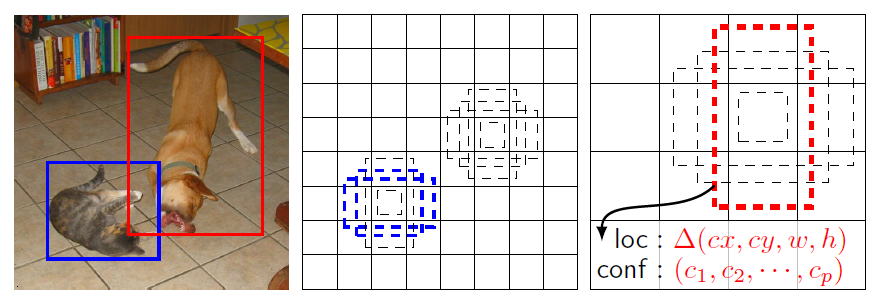
\includegraphics[scale=.5]{ch2/SSD1}
  \end{center}
  Ngoài ra, bằng việc tính toán bounding box trên các feature map khác nhau, tại mỗi tầng feature map, một box sẽ ôm trọn một phần hình ảnh với các kích thước khác nhau. Như trên ví dụ trên, con mèo và con chó có thể được phát hiện ở 2 tầng feature map khác nhau, 2 kích thước và tỉ lệ khác nhau. Thay vì sử dụng 1 box và thay đổi kích thước box cho phù hợp với vật thể, thì SSD dử dụng nhiều box trên nhiều tầng, từ đó tổng hợp ra vị trí và kích thước box kết quả. Bằng việc loại trừ các region proposal, SDD có thể đạt được tốc tộ xử lí cao hơn Faster R-CNN
  \subsubsection{Kiến trúc của SSD}
  \begin{center}
  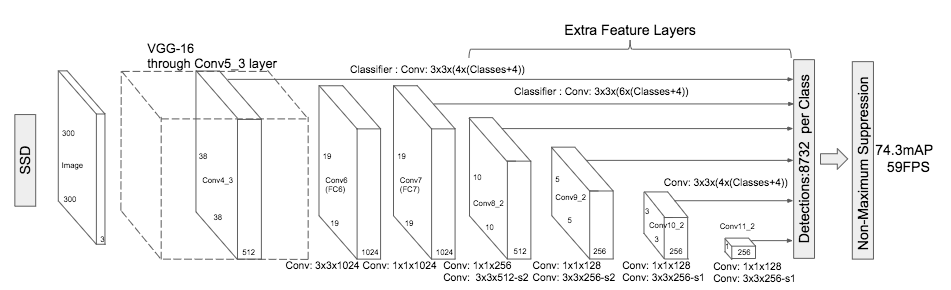
\includegraphics[scale=.5]{ch2/SSD2}
  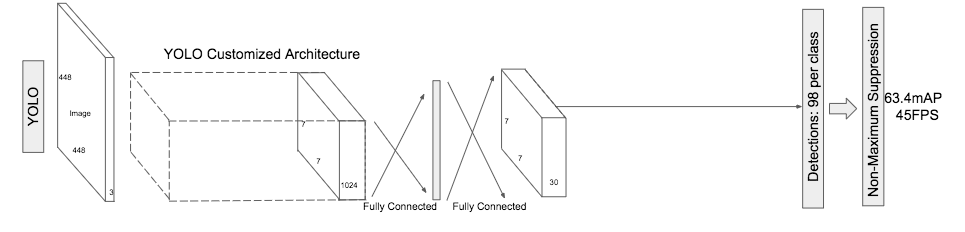
\includegraphics[scale=.5]{ch2/SSD3}
  \end{center}
  Kiến trúc của SSD được xây dựng trên VGG-16 được loại bỏ tầng fully-connected. Lí do mà VGG-16 được sử dụng như tầng cơ sở là vì sự hiệu quả của nó trong bài toán phân loại ảnh với các ảnh có độ phân giải cao. Thay vì sử dụng tầng fully-connected của VGG như của YOLO, một tập các tầng convolution phụ trợ được thêm vào, vì vậy ta có thể trích xuất được các features với nhiều tỉ lệ khác nhau, và giảm gần kích thước của đầu vào trong từng tầng mạng.
  \paragraph{Default boxes}
  \mbox{}\\Trên một feature map kích cỡ \( m \times n\), tại mỗi vị trí cell hay tại mỗi pixel, khởi tạo các default bounding box, các box này có vai trò giống như các anchor của Faster R-CNN. Tuy nhiên, vì vị trí mỗi cell cố định nên các box này cũng sẽ được cố định. Tại mỗi cell, giả sử khởi tạo kk box, SSD tính toán phân loại cc class và đồng thời tính toán xem hình dáng của box như thế nào như toạ độ \((cx,cy)\), dài và rộng \((w,h)\) Vậy tổng số tính toán là \((c+4) k \times m \times n \)

\subsection{Training}
  Việc training SSD yêu cầu cung cấp thông tin về các groundtruth của vật thể bao gồm các thông tin về class, shape.
  \paragraph{Tìm các box phù hợp}
  \mbox{}\\Trong quá trình training, ta tiến hành tìm các default box trên các feature map phù hợp với groundtruth bằng cách tìm các box có Intersection over Union (IoU) cao. Công thức tính IoU dựa trên tỉ lệ giữa diện tích vùng trùng nhau giữa 2 tập và diện tích của cả 2 tập hợp lại
  \begin{center}
  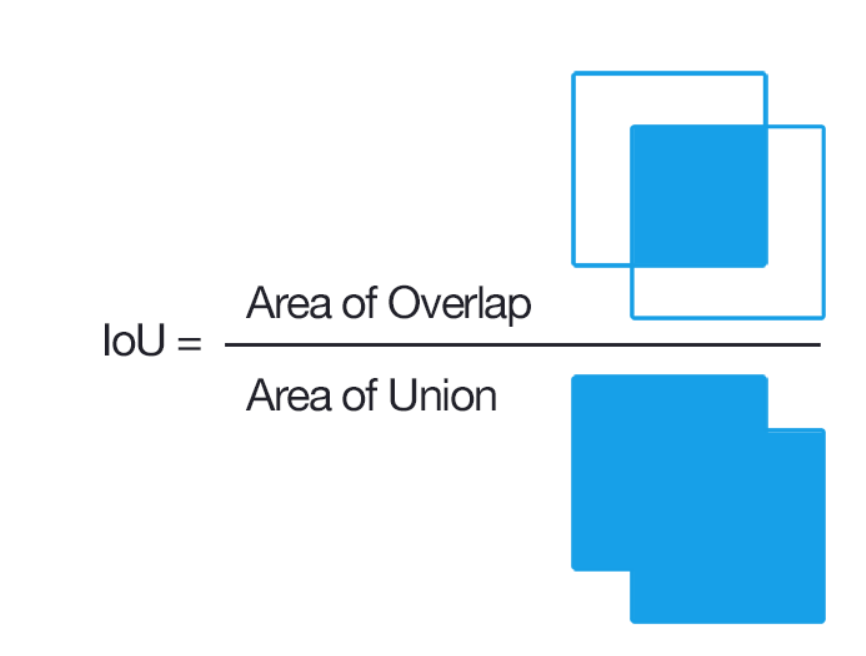
\includegraphics[scale=.5]{ch2/iou}
  \end{center}
  Các box được lọc có chỉ số IoU lớn hơn mức threshol 0.5
  \paragraph{Loss function}
  \mbox{}\\Hàm loss của SSD được xây dựng bằng localization loss để đánh giá việc phát hiện và confidence loss để đánh giá việc phân lớp đối tượng.
  \\Đặt \(x_{ij}^p\) = [1,0] ứng với default box thứ \(i\) khớp với groundtruth thứ \(j\) thuộc lớp \(p\), ta có hàm Loss sau:
  \[L\left( x,c,l,g \right) = \frac{1}{N} \left( L_{conf} \left( x,c \right) + \alpha L_{loc}\left(x,l,g\right)\right)\]
  N ở đây là số lượng những default box phù hợp được tìm ở bước trên. Nếu N = 0 thì Loss = 0. Hàm Loss \(L_{loc}\) được tính bằng Smooth L1 loss giữa box dự đoán \(l\) và groundtruth box \(g\). Với các tham số như điểm chính giữa \(\left(cx,cy\right)\) của default box \(d\) và chiều dài \(w\), chiều rộng \(h\). \(\alpha\) được đặt là 1.
  \paragraph{Localization Loss}
  \mbox{}\[L_{loc}\left( x,l,g \right) = \sum^N_{i\in Pos} \sum_{m\in\{cx,cy,w,h\}} x_{ij}^k smooth_{L1}\left( l_i^m - \hat{g}^m_j\right)\]
  Với:
  \[smooth_{L1} \colon= piewise( abs( x ) < 1, 0.5x^2, abs( x ) - 0.5)\]
  Và:
  \[\hat{g}_j^{cx} = \left( g_j^{cx} - d_j^{cx} \right)/ d_j^w\]
  \[\hat{g}_j^{cy} = \left( g_j^{cy} - d_j^{cy} \right) / d_j^h\]
  \[\hat{g}_j^w = \log\left( \frac{g_j^w}{d_j^w} \right)\]
  \[\hat{g}_j^h = \log\left( \frac{g_j^h}{d^h_i} \right)\]
  \paragraph{Confidence Loss}
  \mbox{}\[L_{conf} \left( x,c \right) = - \sum_{i \in Pos}^N x_{ij}^p \log \left( \hat{c}_i^p \right) - \sum_{i \in N eg} \log\left( \hat{c}_i^p \right)\]
  Với:
  \[\hat{c}_i^p = \frac{\exp\left( c_i^p \right)}{\sum_p \exp\left( c_i^p \right)}\]
  \paragraph{Chọn kích thước và tỉ lệ cho default box}
  \mbox{}\\Các feature map ở độ sâu khác nhau sẽ có kích thước khác nhau, vì vậy, kích thước của các default box cũng được thay đôi theo độ sâu của feature map. Ví dụ với độ sâu là m (bao gồm m feature map tại bước detect):\[s_k = s_{min} + \frac{s_{max} - s_{min}}{m - 1} \left( k - 1 \right), \text{k} \in \left[1,m \right] \text{,} s_{min}=0.2 \text{,} s_{max}=0.9\]
  Vậy với m = 3, ta lần lượt sẽ có \(s_1 = 0.2, s_2 = 0.55, s_3 = 0.9\)
  \\Với tỉ lệ giữa chiều dài và rộng của box, sẽ được tính với \(a_r \in { 1, 2, 3, \frac{1}{2}, \frac{1}{3}}\)
  \\Chiều dài và rộng có thể được tính từ \(a_r\):
  \[w_k^a = s_k \sqrt{a_r}\]
  \[h_k^a = s_k / \sqrt{a_r}\]
  Với trường hợp tỉ lệ bằng 1, ta thêm 1 box nữa với kích thước là \({s\prime}_k = \sqrt{s_ks_k+1}\) Như vậy, trên một vị trí của feature map sẽ có tổng cộgn 6 bounding box. Tâm điểm của mỗi box sẽ được tính bằng:
  \[\left( \frac{i+0.5}{\vert f_k \vert}, \frac{j+0.5}{\vert f_k \vert} \right)\]
  Với \(\vert f_k \vert\) là kích cỡ cửa feature map hình vuông. \(i , j\) là vị trí của cell.

\newpage
\chapter {QUÁ TRÌNH RA QUYẾT ĐỊNH}
\chaptermark{Quá trình ra quyết định}


\section{Tính toán để đưa ra các quyết định}
	Việc đưa ra quyết định của thuật toán phát triển bởi nhóm sẽ dựa vào các dữ liệu đầu vào là tâm của các vật thể đang di động mà mạng trí tuệ nhân tạo trả về sau quá trình xử lý ở phần trên. Vị trí của những tâm vật thể sẽ chứa nhiều thông tin về vị trí tương đối của vật thể so với xe, cụ thể là camera nằm trên xe. Ta sẽ bỏ qua kích thước cụ thể của vật thể trong ảnh, vì việc tính toán chính xác kích thước vật thể sẽ làm phức tạp bài toán hơn và độ chính xác cao đến từ việc tính toán kích thước vật thể cũng không cần thiết trong dự án lần này.

	Ý tưởng của thuật toán quyết định là chia ảnh đầu vào thành các vùng khác nhau và việc tâm vật thể nằm trong vùng nào sẽ ảnh hưởng đến quyết định cuối cùng. Cụ thể, ta chia ảnh ra thành những vùng chính:
	\begin{itemize}
		\item Background: Trong hình ảnh, sẽ tồn tại một phần không phải là đường chạy của xe. Phần này có thể là bầu trời, nhà cao tầng,.... nằm trong hình ảnh thu được bởi camera. Trong dự án này, ta sẽ bỏ qua việc làn đường bị giới hạn. Cụ thể, ta có thể xem xe có thể rẽ phải hoặc rẽ trái tùy ý, mà không xét đến lề đường, nhà cao tầng,... Mục đích cuối cùng là xác định hướng rẽ tránh được vật thể mà không va chạm vật thể khác. Vì thế, những vật thể có tâm nằm trong phần Background sẽ được bỏ qua.

		\item Zone of Interest (ZOI): Vùng không phải là Background sẽ được xem là vùng ZOI. ZOI sẽ được chia ra làm nhiều vùng nhỏ hơn, và việc tâm vật thể nằm trong vùng phụ nào của ZOI sẽ ảnh hưởng đến quyết định của thuật toán.

		\item Right: Vùng nằm bên phải của bức ảnh, vằ nằm trong vùng ZOI. Các tâm vật thể nằm trong vùng này cho thấy rằng bên phải không an toàn, vì có vật thể đang chắn. Việc tồn tại tâm nằm trong vùng này sẽ quyết định xe có được rẽ phải hay không.

		\item Left: Vùng nằm bên trái của bức ảnh, và nằm trong vùng ZOI. Tương tự như vùng Right, tồn tại tâm vật thể nằm trong vùng Left có nghĩa là việc rẽ trái là cần phải cân nhắc.

		\item Dodge: Nằm giữa bức ảnh, và nằm trong vùng ZOI. Vật thể nằm trong vùng này hàm ý rằng đường đi đang bị cản trở, và xe sẽ phải ra quyết định rẽ trái, rẽ phải, hoặc đi chậm lại. Việc phương tiện ưu tiên rẽ phải hoặc rẽ phải sẽ tùy thuộc vào tâm vật thể đó nằm trong phần nào của vùng Dodge. Cụ thể, ta chia vùng Dodge ra thành hai vùng Left Refer và Right Refer. Nếu vật thể nằm trong vùng Left Refer, phương tiện sẽ phải rẽ trái và tương tự, nếu vật thể nằm trong Right Refer thì phương tiện sẽ phải rẽ phải. 

	\end{itemize}		
Việc phân chia các vùng có thể được minh họa cụ thể một cách khái quát bằng Hình.\ref{fig:zones}
		\begin{figure}[h]
 		\label{fig:zones}
		\begin{center}
		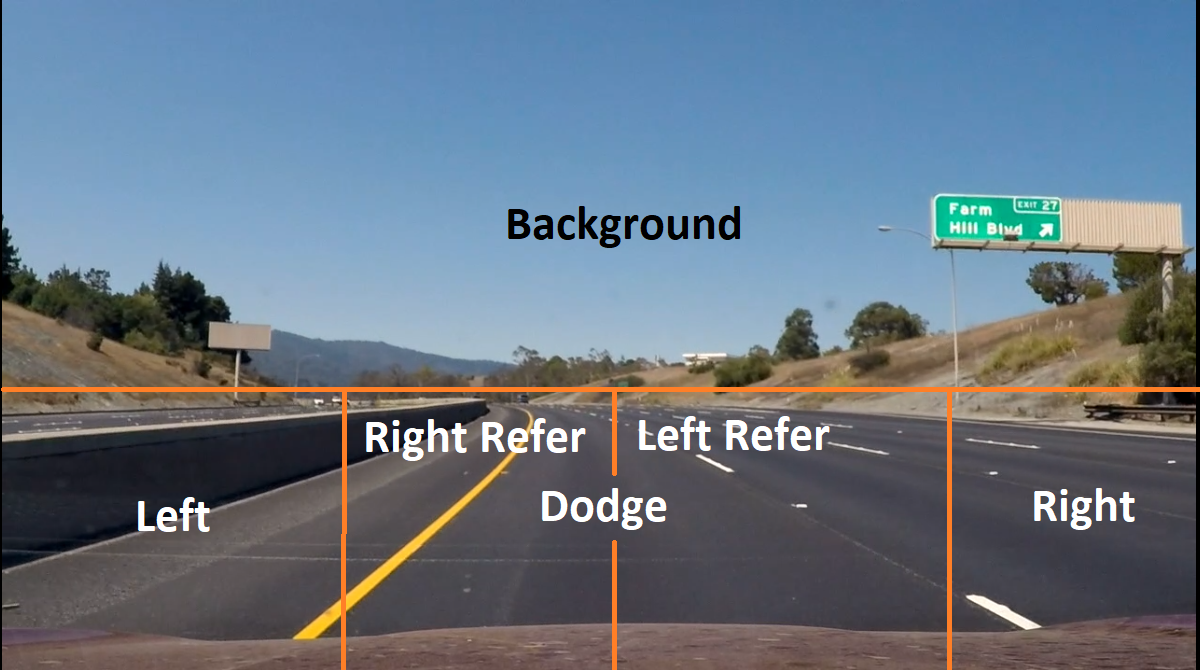
\includegraphics[width=.8\textwidth]{ch3/zones.png} % Include the image placeholder.png
		\caption{Phân vùng hình ảnh}
		\end{center}
		\end{figure}	

Sau khi nhận được tọa độ tâm của các vật thể, bằng việc xem xét vị trí tương ứng của từng tâm rơi vào vùng nào, thuật toán sẽ đưa ra quyết. Nhóm đề ra giải thuật như sau:

	\begin{enumerate}
		\item Kiểm tra có tồn tại vật thể trong vùng Dodge hay không? Nếu không có, tiếp tục đi thẳng và xét tiếp các tâm vật thể khác.
		\item Nếu tồn tại ít nhất một vật thể trong vùng Dodge, xác định xem tâm đó nằm trong phần nào của vùng Dodge (Left Refer hoặc Right Refer).
		\item Nếu vật thể nằm trong vùng Left Refer, ta kiểm tra xem bên vùng Left có tồn tại vật thể nào hay không. Nếu có, ta cho phương tiện chạy chậm lại, nếu không, ta cho phương tiện rẽ trái.
		\item Nếu vật thể nằm trong vùng Right Refer, ta kiểm tra xem vùng Right có tồn tại vật thể hay không. Nếu có, ta cho phương tiện chạy chậm lại, nếu không, ta cho phương tiện rẽ trái.	
	\end{enumerate}
Thuật toán được minh họa bằng sơ đồ giải thuật trong Hình.\ref{fig:flowchart}.

		\begin{figure}[h]
 		\label{fig:flowchart}
		\begin{center}
		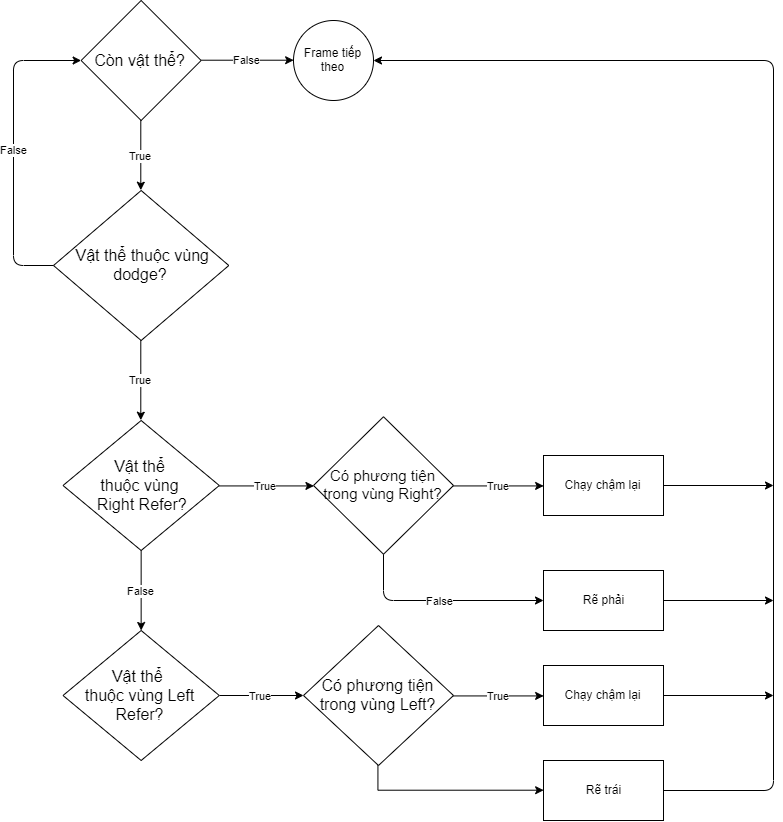
\includegraphics[width=.8\textwidth]{ch3/algo-flowchart.png} % Include the image placeholder.png
		\caption{Giải thuật ra quyết định}
		\end{center}
		\end{figure}	

\newpage
\chapter {CÁC THỬ NGHIỆM VÀ KẾT QUẢ}
\chaptermark{Các thử nghiệm và kết quả}

\section{KTIT dataset}

\newpage
\chapter {KẾT LUẬN}
\chaptermark{Kết luận}

\section{Nhận xét}

\section{Hướng phát triển sau này}


\newpage



%%% Document ending contents -----------------------------------
\renewcommand\bibname{TÀI LIỆU THAM KHẢO}
\nocite{*}
\bibliography{references}\cleardoublepage
\bibliographystyle{ieeetr}
\newpage


\end{document}



